\documentclass[11pt,compress,t,notes=noshow]{beamer}\usepackage[]{graphicx}\usepackage[]{color}

\makeatletter
\def\maxwidth{ %
  \ifdim\Gin@nat@width>\linewidth
    \linewidth
  \else
    \Gin@nat@width
  \fi
}
\makeatother

\definecolor{fgcolor}{rgb}{0.345, 0.345, 0.345}
\newcommand{\hlnum}[1]{\textcolor[rgb]{0.686,0.059,0.569}{#1}}%
\newcommand{\hlstr}[1]{\textcolor[rgb]{0.192,0.494,0.8}{#1}}%
\newcommand{\hlcom}[1]{\textcolor[rgb]{0.678,0.584,0.686}{\textit{#1}}}%
\newcommand{\hlopt}[1]{\textcolor[rgb]{0,0,0}{#1}}%
\newcommand{\hlstd}[1]{\textcolor[rgb]{0.345,0.345,0.345}{#1}}%
\newcommand{\hlkwa}[1]{\textcolor[rgb]{0.161,0.373,0.58}{\textbf{#1}}}%
\newcommand{\hlkwb}[1]{\textcolor[rgb]{0.69,0.353,0.396}{#1}}%
\newcommand{\hlkwc}[1]{\textcolor[rgb]{0.333,0.667,0.333}{#1}}%
\newcommand{\hlkwd}[1]{\textcolor[rgb]{0.737,0.353,0.396}{\textbf{#1}}}%
\let\hlipl\hlkwb

\usepackage{framed}
\makeatletter
\newenvironment{kframe}{%
 \def\at@end@of@kframe{}%
 \ifinner\ifhmode%
  \def\at@end@of@kframe{\end{minipage}}%
  \begin{minipage}{\columnwidth}%
 \fi\fi%
 \def\FrameCommand##1{\hskip\@totalleftmargin \hskip-\fboxsep
 \colorbox{shadecolor}{##1}\hskip-\fboxsep
     \hskip-\linewidth \hskip-\@totalleftmargin \hskip\columnwidth}%
 \MakeFramed {\advance\hsize-\width
   \@totalleftmargin\z@ \linewidth\hsize
   \@setminipage}}%
 {\par\unskip\endMakeFramed%
 \at@end@of@kframe}
\makeatother

\definecolor{shadecolor}{rgb}{.97, .97, .97}
\definecolor{messagecolor}{rgb}{0, 0, 0}
\definecolor{warningcolor}{rgb}{1, 0, 1}
\definecolor{errorcolor}{rgb}{1, 0, 0}
\definecolor{code}{rgb}{0.97, 0.96, 1.0}
\newenvironment{knitrout}{}{} % an empty environment to be redefined in TeX

\usepackage{alltt}
\usepackage[utf8]{inputenc}
\usepackage[ngerman]{babel}
\usepackage{dsfont}
\usepackage{verbatim}
\usepackage{amsmath}
\usepackage{amsfonts}
\usepackage{mathtools}
\usepackage{csquotes}
\usepackage{cmbright}
\usepackage{multirow}
\usepackage{longtable}
\usepackage{enumerate}
\usepackage[absolute,overlay]{textpos}
\usepackage{psfrag}
\usepackage{algorithm}
\usepackage{algpseudocode}
\usepackage{eqnarray}
\usepackage{bytefield}
\usepackage{animate}
\usepackage{tikz}
\usetikzlibrary{shapes,matrix,positioning,chains,arrows,shadows,decorations.pathmorphing,fit,backgrounds}
\usepackage{adjustbox}
\usepackage{colortbl}
\usepackage{tabularx} % for tables (incl. \hline)
\usepackage{arydshln} % Load after array, longtable, colortab and/or colortbl , otherwise problems with \hline in tabular env
\usepackage{etex} %increase registers for \dimenS to more than 256, otherwise we get "No room for a new \dimen"
\usepackage{graphicx}
\usepackage{booktabs} %used in epr lectures
\usepackage{bm} % bold greek letters
\usepackage{hyperref} % url citing
\usepackage{blkarray} % block arrays
\usepackage{listings} % block of code
\usepackage{xcolor} %colored math symbols
\usepackage{pgffor}
\usepackage{verbatimbox}
\usepackage{xcolor}

%some colors
\definecolor{checkgreen}{HTML}{18A126}
\definecolor{errorred}{HTML}{FF0000}
\definecolor{blockbg}{HTML}{F7F7F7}
\definecolor{gray}{HTML}{A0A0A0}

% basic latex stuff
\newcommand{\col}{\par\colorbox{code}{\parbox{\textwidth}{\theverbbox}}\par}
\newcommand{\eg}{e.\,g.\xspace} %for example
\newcommand{\ie}{i.\,e.\xspace} %that is to say...
\newcommand{\pkg}[1]{{\fontseries{b}\selectfont #1}} %fontstyle for R packages
\newcommand{\lz}{\vspace{0.5cm}} %vertical space
\newcommand{\oneliner}[1] % Oneliner for important statements
{\begin{block}{}\begin{center}\begin{Large}#1\end{Large}\end{center}\end{block}}
\def\SpAr{\quad \Rightarrow \quad}

%new environments
\newenvironment{vbframe}  %frame with breaks and verbatim
{
 \begin{frame}[containsverbatim,allowframebreaks]
}
{
\end{frame}
}

\newenvironment{vframe}  %frame with verbatim without breaks (to avoid numbering one slided frames)
{
 \begin{frame}[containsverbatim]
}
{
\end{frame}
}

\newenvironment{blocki}[1]   % itemize block
{
 \begin{block}{#1}\begin{itemize}
}
{
\end{itemize}\end{block}
}

\newenvironment{fragileframe}[2]{  %fragile frame with framebreaks
\begin{frame}[allowframebreaks, fragile, environment = fragileframe]
\frametitle{#1}
#2}
{\end{frame}}

\newcommand{\myframe}[2]{  %short for frame with framebreaks
\begin{frame}[allowframebreaks]
\frametitle{#1}
#2
\end{frame}}

\usepackage{../../style/lmu-lecture}

\let\code=\texttt
\let\proglang=\textsf

\setkeys{Gin}{width=0.9\textwidth}

\usepackage{tikz}
\usetikzlibrary{shapes,arrows,snakes, calc}

% Define block styles
\tikzstyle{decision} = [diamond, draw, text width=6em, text badly centered, node distance=4cm, inner sep=0pt]
\tikzstyle{decision2} = [diamond, draw, fill=customgreen!35, text width=6em, text badly centered, node distance=4cm, inner sep=0pt]

\tikzstyle{block} = [rectangle, draw, text width=14em, text centered, rounded corners, node distance=3cm, minimum height=4em]
\tikzstyle{line} = [draw, -latex']
\tikzstyle{cloud} = [draw, ellipse, node distance=3cm, minimum height=2em]

\title{Introduction to Deep Learning}
\author{Bernd Bischl}
\institute{Department of Statistics -- LMU Munich}
\date{WS 2021/2022}

\setbeamertemplate{frametitle}{\expandafter\uppercase\expandafter\insertframetitle}

\IfFileExists{upquote.sty}{\usepackage{upquote}}{}
\input{../../latex-math/basic-math}
\input{../../latex-math/basic-ml}
\input{../../latex-math/ml-nn}

\begin{document}

\lecturechapter{2}{MLP -- Matrix Notation}
\lecture{MLP -- Matrix Notation}
%%%%%%%%%%%%%%%%%%%%%%%%%%%%%%%%%%%%%%%%%%%%%%%%%%%%%%%%%%%%%%%%%%

\begin{frame}
\frametitle{Lecture outline}
\lz
This chapter introduces a compact way for representing feedforward neural networks: the matrix formalism from linear algebra.
\lz
\lz

\begin{enumerate}
\item First, we explore networks with one hidden layer and one output unit.
\lz
\item Next, we investigate networks with one hidden layer but multiple output units.
\lz
\item Finally, we focus on multi-layer feedforward networks with an arbitrary number of hidden layers and output units.
\end{enumerate}
\end{frame}
%%%%%%%%%%%%%%%%%%%%%%%%%%%%%%%%%%%%%%%%%%%%%%%%%%%%%%%%%%%%%%%%%%

\section{Single Hidden Layer Networks for Regression and Binary Classification}
%%%%%%%%%%%%%%%%%%%%%%%%%%%%%%%%%%%%%%%%%%%%%%%%%%%%%%%%%%%%%%%%%%

\begin{vbframe}{Single Hidden Layer Networks}

\begin{itemize}
\item The input $\xv$ is a column vector with dimensions $p \times 1$. 
\item $\Wmat$ is a weight matrix with dimensions $p \times m$:
$$\Wmat =
     \begin{pmatrix}
      w_{1,1} & w_{1,2} & \cdots & w_{1,m} \\
      w_{2,1} & w_{2,2} & \cdots & w_{2,m} \\
      \vdots  & \vdots  & \ddots & \vdots  \\
      w_{p,1} & w_{p,2} & \cdots & w_{p,m}
     \end{pmatrix}$$
\item For example, to obtain $z_1$, we pick the first column of $W$:
    $$\Wmat_1 =
     \begin{pmatrix}
      w_{1,1} \\
      w_{2,1} \\
      \vdots  \\
      w_{p,1}
     \end{pmatrix}$$
and compute $z_1 = \sigma(W_1^\top \xv + b_1)$, where $b_1$ is the bias of the first hidden neuron and $\sigma: \R \to \R$ is an activation function. 
\end{itemize}
\end{vbframe}
%%%%%%%%%%%%%%%%%%%%%%%%%%%%%%%%%%%%%%%%%%%%%%%%%%%%%%%%%%%%%%%%%%

\begin{vbframe}{Single Hidden Layer Networks: Notation}
  \textbf{General notation}:
  \begin{itemize}
    \vspace{4mm}
    \item The network has $m$ hidden neurons $z_1, \dots, z_m$ with
    $$ z_j = \sigma(\Wmat_j^\top \xv + b_j)$$
    \vspace{-0.5cm}
    \begin{itemize}
    \item $z_{in,j}  = \Wmat_j^\top \xv + b_j$
    \vspace{2mm}
    \item $z_{out,j} = \sigma(z_{in,j}) = \sigma(\Wmat_j^\top \xv + b_j)$
    \end{itemize}
    \vspace{4mm}
    for $j \in \{1,\ldots,m\}$.
    \vspace{4mm}
    \framebreak 
%%%%%%%%%%%%%%%%%%%%%%%%%%%%%%%%%%%%%%%%%%%%%%%%%%%%%%%%%%%%%%%%%%

\item Vectorized notation:
\begin{itemize}
\item $ \hidz_{in} = (z_{in,1}, \dots, z_{in,m})^\top = \Wmat^\top \xv + \biasb$ \\ (Note: $\Wmat^\top \xv$ = $(\xv^\top \Wmat)^\top$)
\item $ \hidz = \hidz_{out} = \sigma(\hidz_{in}) = \sigma(\Wmat^\top \xv + \biasb)$, where the (hidden layer) activation function $\sigma$ is applied element-wise to $\hidz_{in}$.  
\end{itemize}
\item Bias term:         
\begin{itemize}
\item We sometimes omit the bias term by adding a constant feature to the input $\tilde{\xv} = (1, x_1, ..., x_p)$ and by adding the bias term to the weight matrix 
$$\tilde{\Wmat} = (\biasb, \Wmat_1, ..., \Wmat_p).$$ 
\item \textbf{Note}: For simplification purposes, we will not explicitly represent the bias term graphically in the following. However, the above \enquote{trick} makes it straightforward to represent it graphically. 
\end{itemize}
\end{itemize}
\framebreak
%%%%%%%%%%%%%%%%%%%%%%%%%%%%%%%%%%%%%%%%%%%%%%%%%%%%%%%%%%%%%%%%%%

  \textbf{General notation}:
  \begin{itemize}
    \vspace{4mm}
    \item For regression or binary classification: one output unit $f$ where
      \begin{itemize}
        \item $f_{in} = \wtu^\top \hidz + c$ , i.e. a linear combination of derived features plus the bias term $c$ of the output neuron, and
        \vspace{2mm}
        \item $f(\xv)= f_{out} = \tau(f_{in}) = \tau(\wtu^\top \hidz + c)$ , where $\tau$ is the output activation function.
      \end{itemize}
    \item For regression $\tau$ is the identity function.
    \item For binary classification, $\tau$ is a sigmoid function.
    \item \textbf{Note}: The purpose of the hidden-layer activation function $\sigma$ is to introduce non-linearities so that the network is able to learn complex functions whereas the purpose of $\tau$ is merely to get the final score on the same scale as the target.
  \end{itemize}

\framebreak 
%%%%%%%%%%%%%%%%%%%%%%%%%%%%%%%%%%%%%%%%%%%%%%%%%%%%%%%%%%%%%%%%%%

  \textbf{General notation: Multiple inputs}
  \begin{itemize}
    \item It is possible to feed multiple inputs to a neural network simultaneously.
    \vspace{2mm}
    \item The inputs $\xi$, for $i \in \nset$, are arranged as rows in the \textbf{design matrix} $\Xmat$.
    \begin{itemize}
      \item $\Xmat$ is a ($n \times p$)-matrix.
    \end{itemize}
    \vspace{2mm}
    \item The weighted sum in the hidden layer is now computed as $\Xmat\Wmat + \bm{B}$, where,
      \begin{itemize}
        \item $\Wmat$, as usual, is a ($p \times m$) matrix, and,
        \vspace{2mm}
        \item $\bm{B}$ is a ($n \times m$) matrix containing the bias vector $\biasb$ (duplicated) as the rows of the matrix.
      \end{itemize}
    \vspace{2mm}
    \item The \textit{matrix} of hidden activations $\bm{Z} = \sigma(\Xmat\Wmat + \bm{B})$
    \begin{itemize}
      \item $\bm{Z}$ is a ($n \times m$) matrix.
    \end{itemize}
  \end{itemize}

\framebreak
%%%%%%%%%%%%%%%%%%%%%%%%%%%%%%%%%%%%%%%%%%%%%%%%%%%%%%%%%%%%%%%%%%

  \begin{itemize}
    \vspace{15mm}
    \item The final output of the network, which contains a prediction for each input, is $\tau(\bm{Z}\wtu + \bm{C})$, where
      \begin{itemize}
        \vspace{2mm}
        \item $\wtu$ is the vector of weights of the output neuron, and,
        \vspace{2mm}
        \item $\bm{C}$ is a ($n \times 1$) matrix whose elements are the (scalar) bias $c$ of the output neuron.
      \end{itemize}
  \end{itemize}
\end{vbframe}
%%%%%%%%%%%%%%%%%%%%%%%%%%%%%%%%%%%%%%%%%%%%%%%%%%%%%%%%%%%%%%%%%%

\begin{frame} {Single Hidden Layer Networks: Example}
  \begin{itemize}
    \item Weights (and biases) of the network.
  \begin{figure}
    \centering
      \only<1>{\scalebox{1}{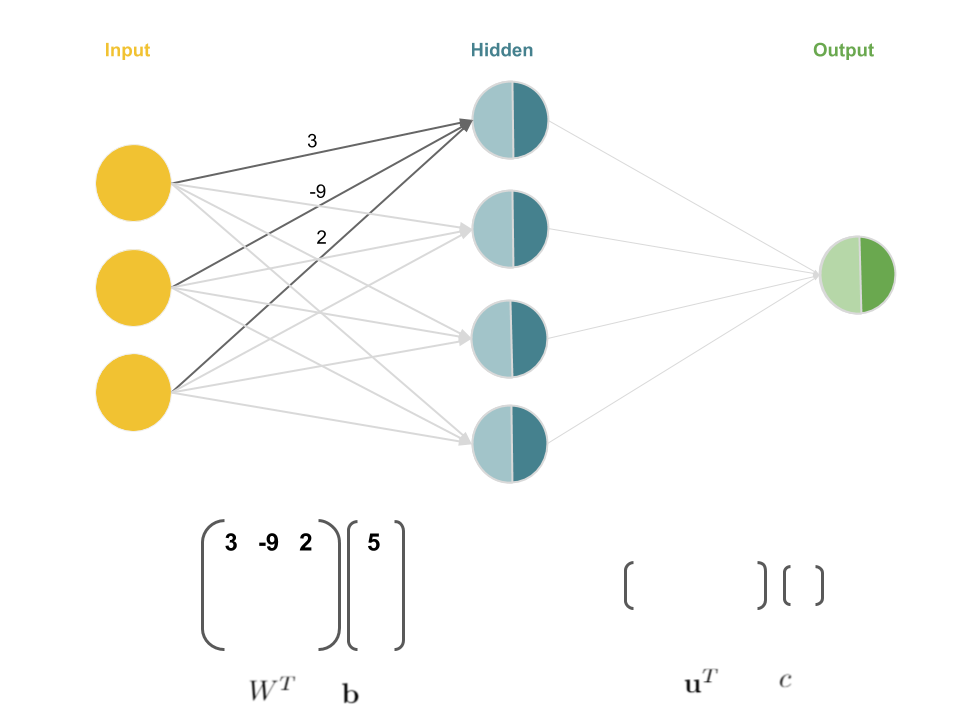
\includegraphics{figure/sinlay_one.png}}}
      \only<2>{\scalebox{1}{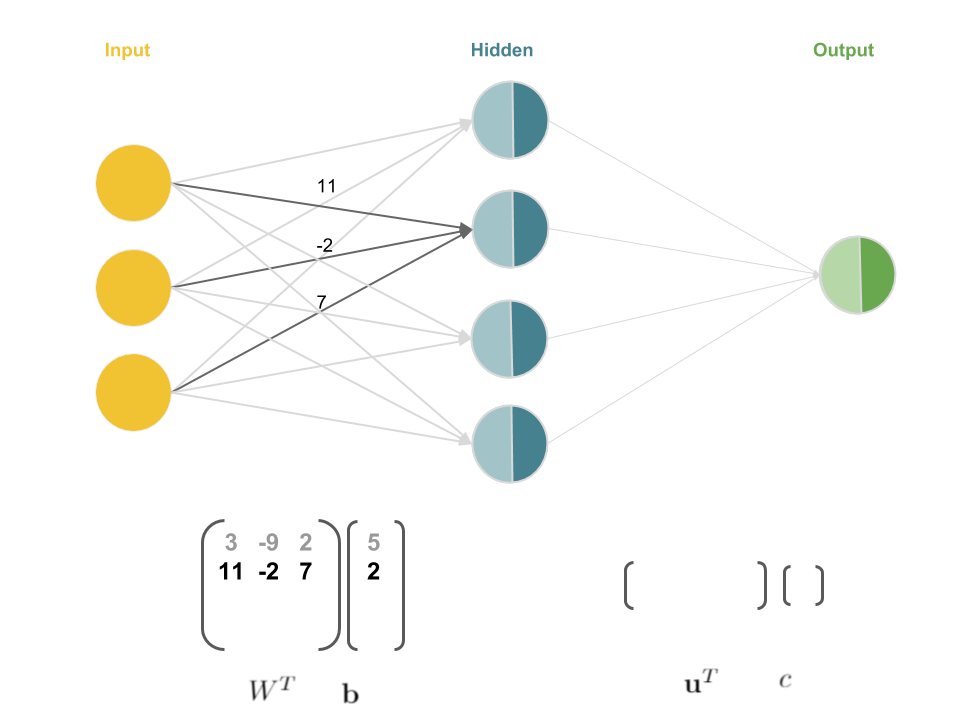
\includegraphics{figure/sinlay_two.png}}}
      \only<3>{\scalebox{1}{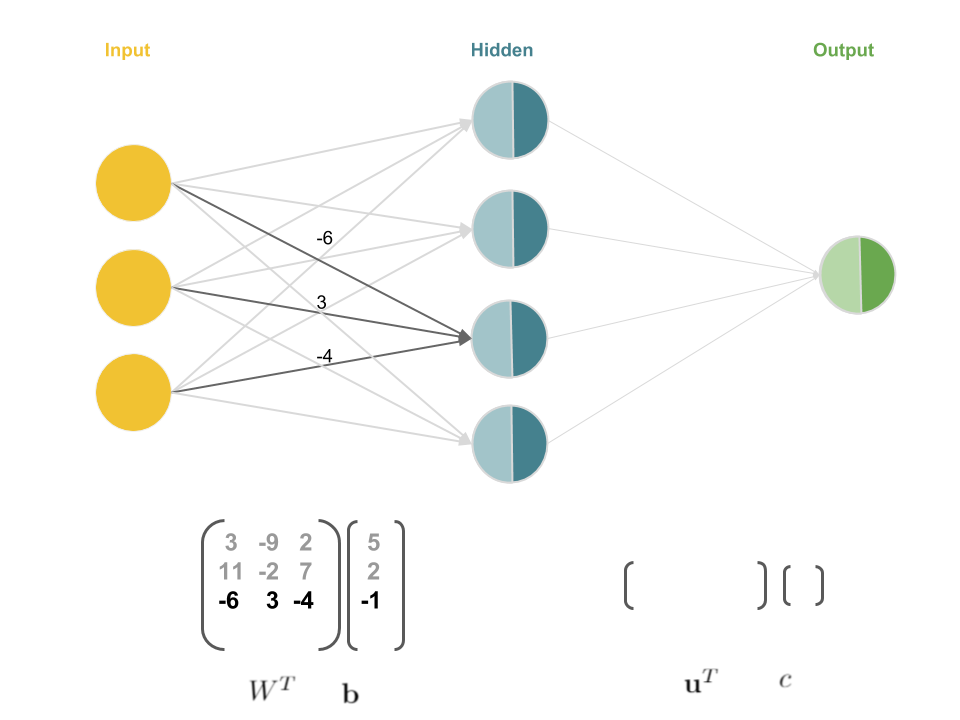
\includegraphics{figure/sinlay_three.png}}}
      \only<4>{\scalebox{1}{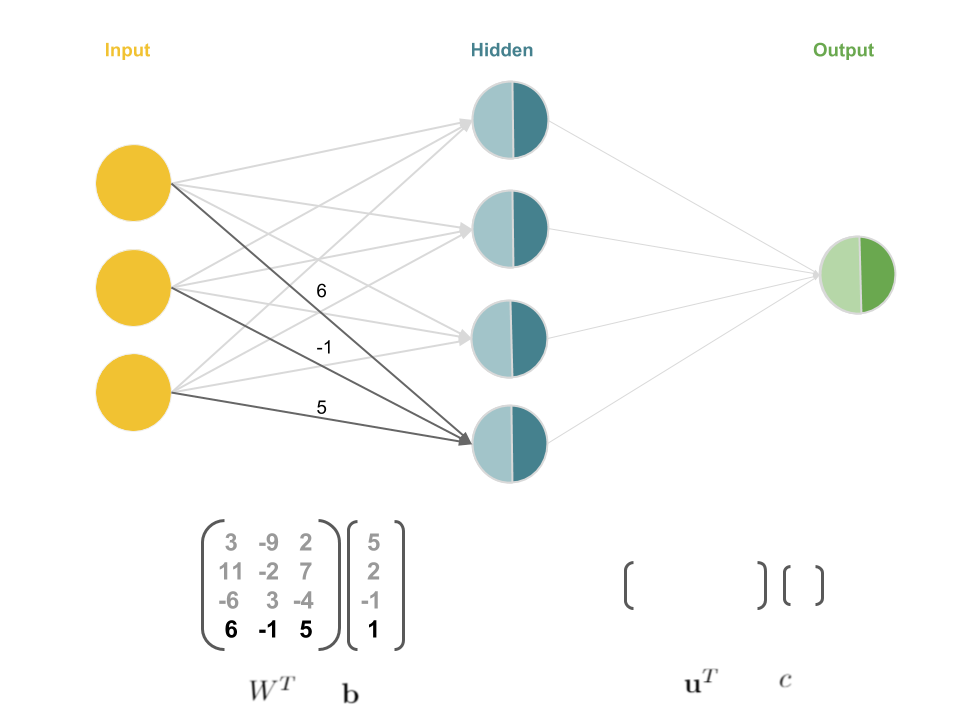
\includegraphics{figure/sinlay_four.png}}}
      \only<5>{\scalebox{1}{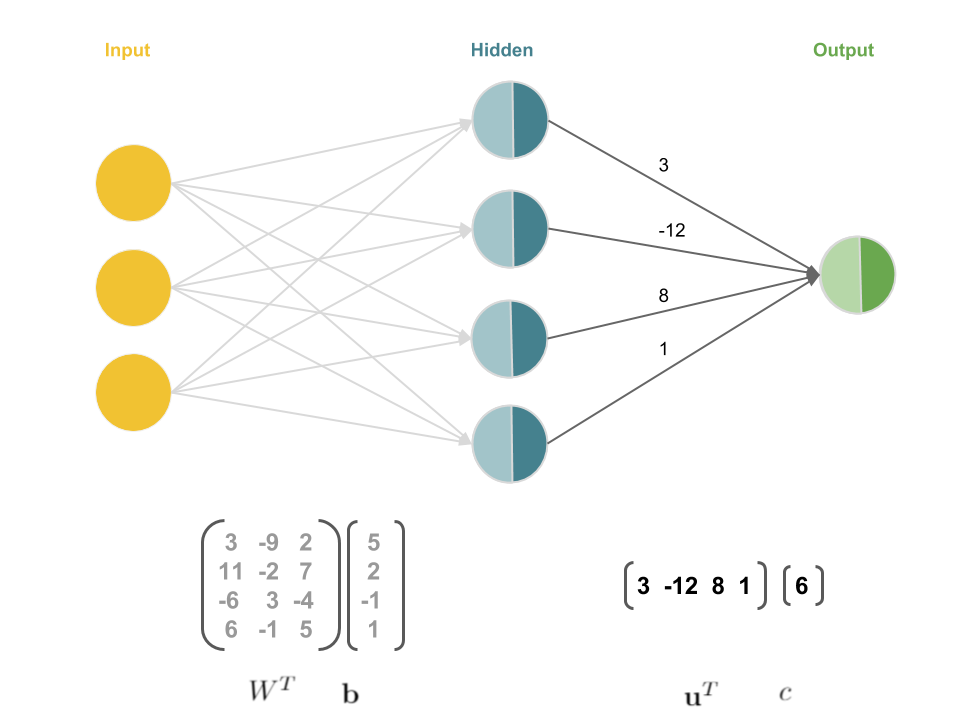
\includegraphics{figure/sinlay_five.png}}}
      \only<6>{\scalebox{1}{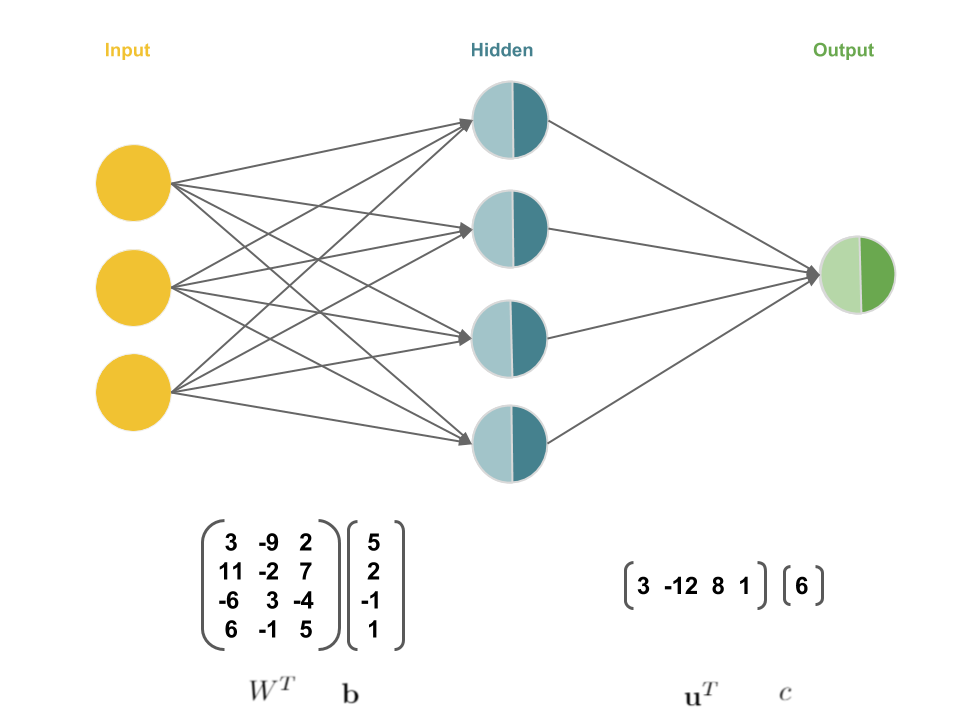
\includegraphics{figure/sinlay_six.png}}}
  \end{figure}
  \begin{figure}
    \centering
  \end{figure}
  \end{itemize}
\end{frame}
%%%%%%%%%%%%%%%%%%%%%%%%%%%%%%%%%%%%%%%%%%%%%%%%%%%%%%%%%%%%%%%%%%

\begin{frame} {Single Hidden Layer Networks: Example}
  
  \small{Forward pass through the shallow neural network.}
  \begin{figure}
    \centering
    \only<1>{\scalebox{1}{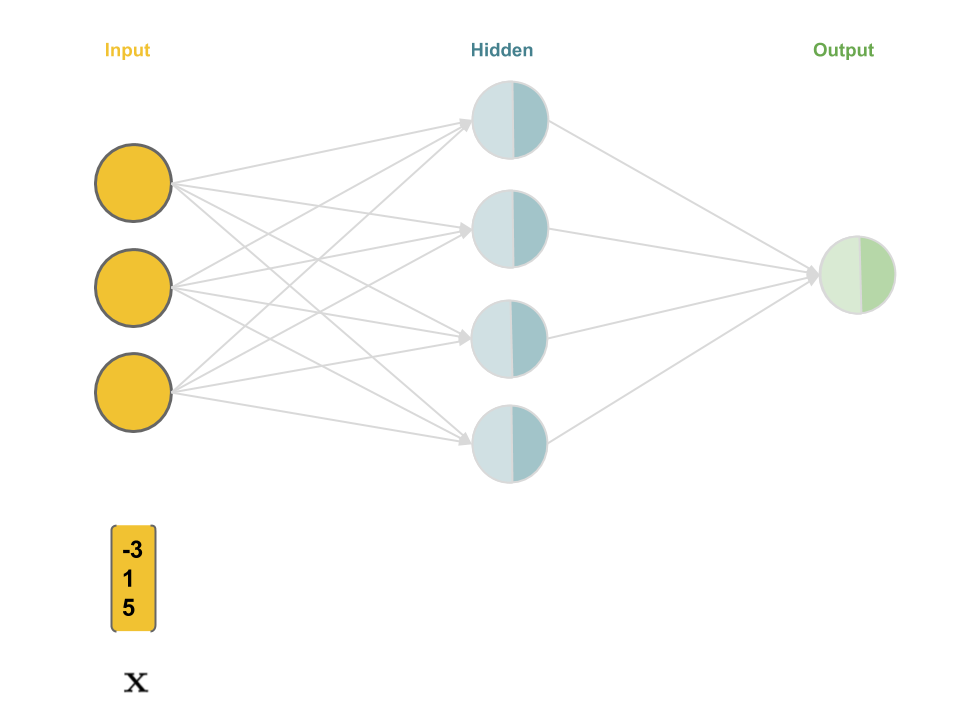
\includegraphics{figure/sinlay_seven.png}}}
    \only<2>{\scalebox{1}{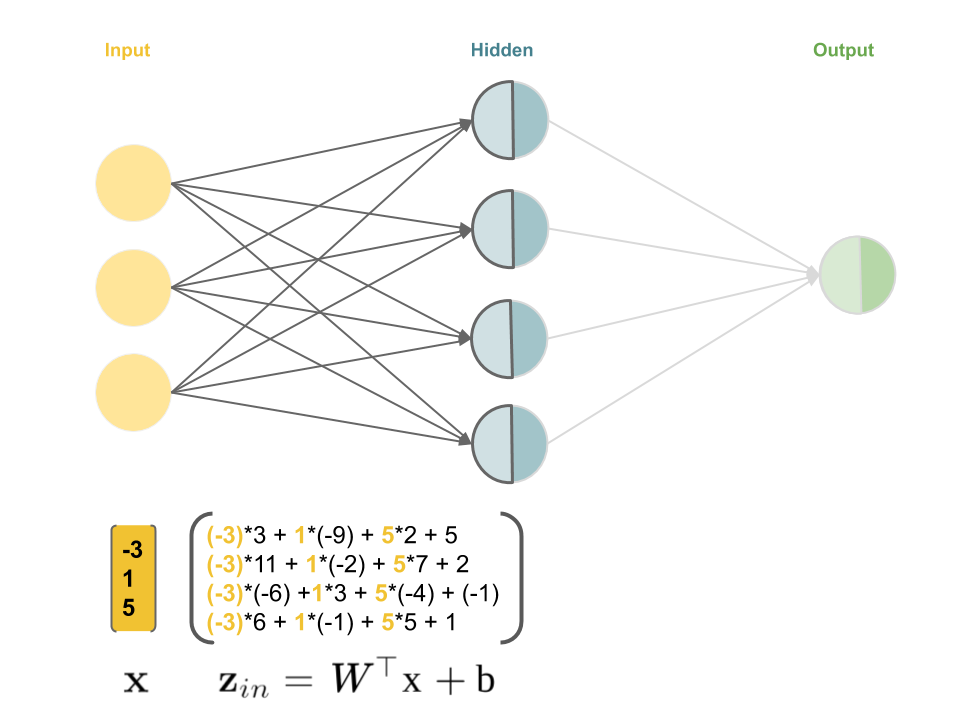
\includegraphics{figure/sinlay_eight.png}}}
    \only<3>{\scalebox{1}{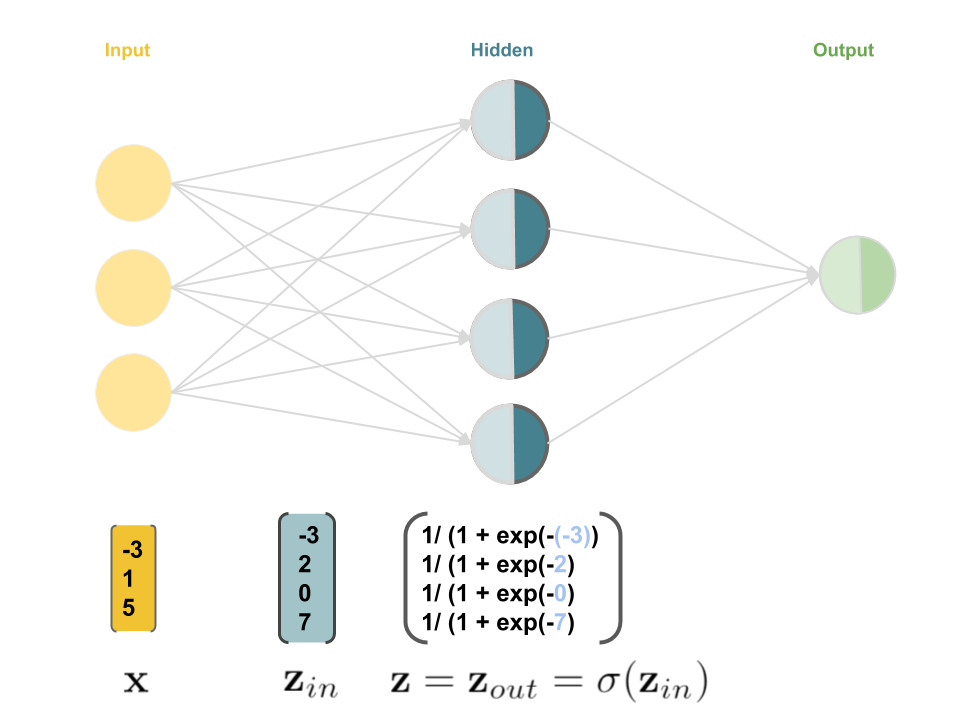
\includegraphics{figure/sinlay_nine.png}}}
    \only<4>{\scalebox{1}{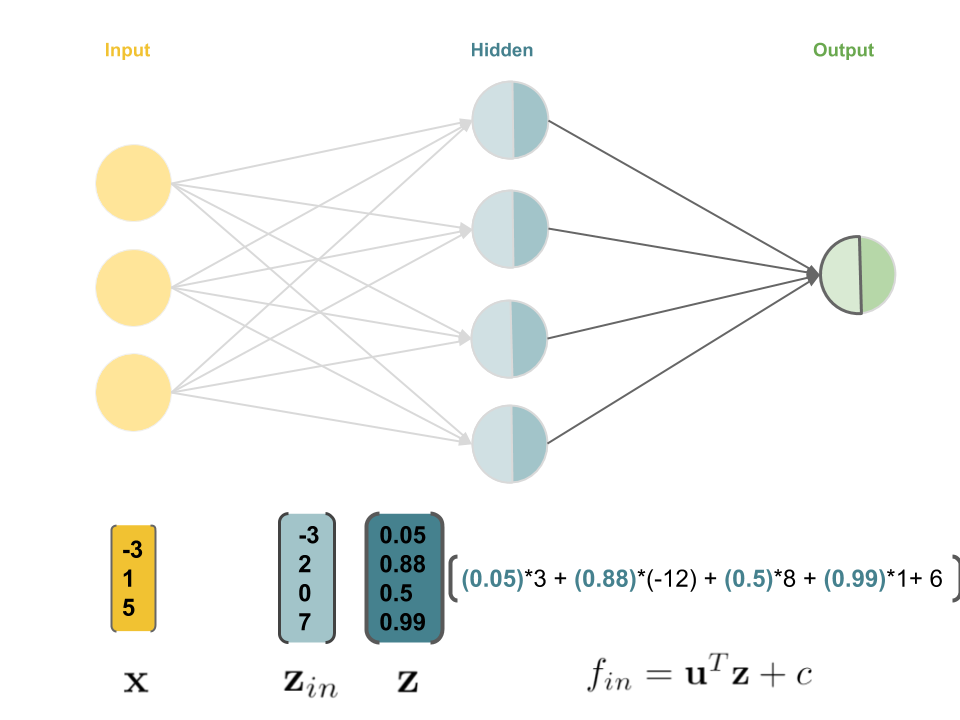
\includegraphics{figure/sinlay_ten.png}}}
    \only<5>{\scalebox{1}{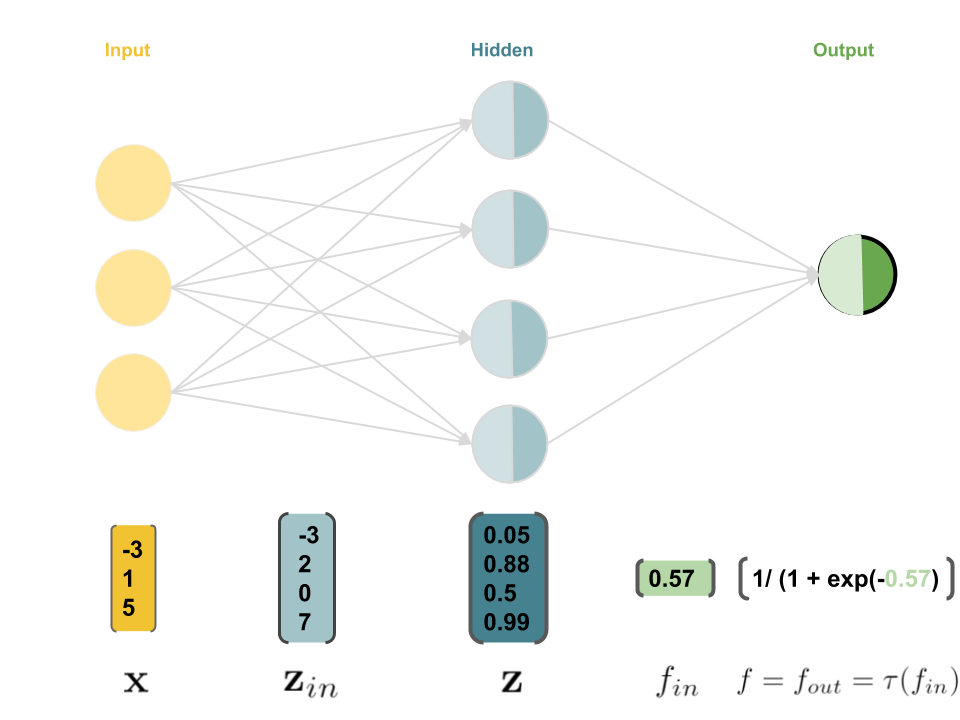
\includegraphics{figure/sinlay_eleven.png}}}
    \only<6>{\scalebox{1}{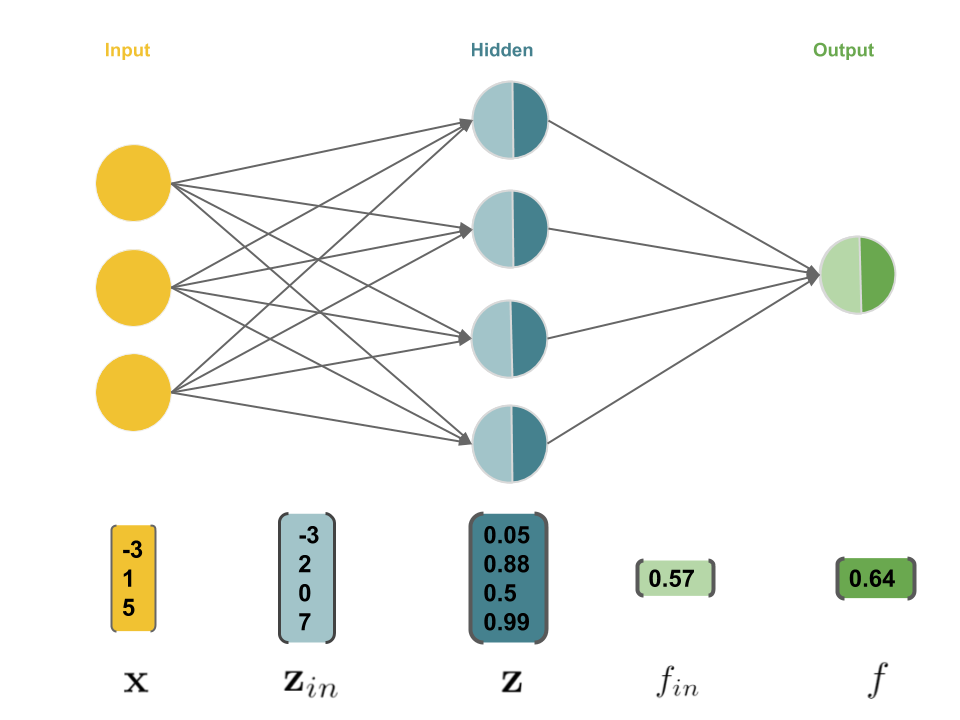
\includegraphics{figure/sinlay_twelve.png}}}
  \end{figure}
\end{frame}
%%%%%%%%%%%%%%%%%%%%%%%%%%%%%%%%%%%%%%%%%%%%%%%%%%%%%%%%%%%%%%%%%%

\begin{frame} {Hidden Layer: Activation Function}
\begin{itemize}
\item It is important to note that if the hidden layer does not have a non-linear activation, the network can only learn linear decision boundaries.
\item For simplification purposes, we drop the bias terms in notation and let $\sigma = \text{id}$. Then:
    \begin{eqnarray*}
        f(\xv) & = & \tau(\wtu^\top \hidz) = \tau(\wtu^\top \sigma(\Wmat^\top \xv)) \\
         & = & \tau(\wtu^\top \sigma(\Wmat^\top \xv)) \\
         & = & \tau(\wtu^\top\Wmat^\top \xv) = \tau(\mathbf{v}^\top \xv)
      \end{eqnarray*}
      where $ \mathbf{v} = \Wmat\wtu$. It can be seen that $f(\xv)$ can only yield a linear decision boundary.
  \end{itemize}
\end{frame}
%%%%%%%%%%%%%%%%%%%%%%%%%%%%%%%%%%%%%%%%%%%%%%%%%%%%%%%%%%%%%%%%%%

%%%%%%%%%%%%%%%%%%%%%%%%%%%%%%%%%%%%%%%%%%%%%%%%%%%%%%%%%%%%%%%%%%
\section{Single Hidden Layer Networks for Multi-Class Classification}
%%%%%%%%%%%%%%%%%%%%%%%%%%%%%%%%%%%%%%%%%%%%%%%%%%%%%%%%%%%%%%%%%%

\begin{frame} {Multi-class Classification}
\vspace{20mm}
\begin{itemize}
\item We have only considered regression and binary classification problems so far.
\vspace{5mm}
\item How can we get a neural network to perform multiclass classification?
  \end{itemize}
\end{frame}
%%%%%%%%%%%%%%%%%%%%%%%%%%%%%%%%%%%%%%%%%%%%%%%%%%%%%%%%%%%%%%%%%%

\begin{frame} {Multi-class Classification}
\begin{itemize}
\item The first step is to add additional neurons to the output layer.
\item Each neuron in the layer will represent a specific class (number of neurons in the output layer = number of classes).
\begin{figure}
\centering
\scalebox{0.75}{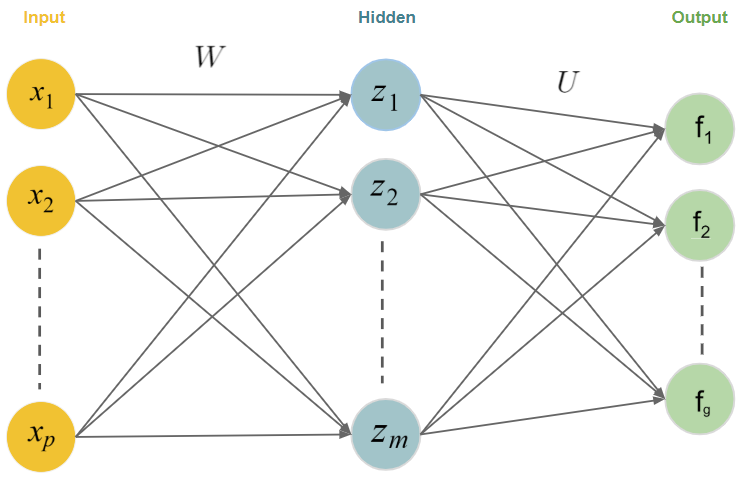
\includegraphics[width=10.2cm]{figure/neuralnet_new.png}}
\caption{\footnotesize Structure of a single hidden layer, feed-forward neural network for g-class classification problems (bias term omitted).}
\end{figure}
\end{itemize}
\end{frame}
%%%%%%%%%%%%%%%%%%%%%%%%%%%%%%%%%%%%%%%%%%%%%%%%%%%%%%%%%%%%%%%%%%

\begin{frame} {Multi-class Classification}
\vspace{5mm}
\begin{blocki}{Notation:}
\item For $g$-class classification, $g$ output units: $$\mathbf{f} = (f_1, \dots, f_g)$$
\vspace{4mm}
\item $m$ hidden neurons $z_1, \dots, z_m$, with
    $$ z_j = \sigma(\Wmat_j^\top \xv), \quad j = 1,\ldots,m. $$
\item Compute linear combinations of derived features $z$:
    $$ f_{in,k} = \bm{U}_k^\top \hidz, \quad \hidz=(z_1,\dots, z_m)^\top, \quad k = 1,\ldots,g$$
\end{blocki}
\end{frame}
%%%%%%%%%%%%%%%%%%%%%%%%%%%%%%%%%%%%%%%%%%%%%%%%%%%%%%%%%%%%%%%%%%

\begin{frame} {Multi-class Classification}
  \begin{itemize}
    \item The second step is to apply a softmax activation function to the output layer.
    \vspace{4mm}
    \item This gives us a probability distribution over $g$ different possible classes:
    $$ f_{out,k} = \tau_k(f_{in,k}) = \frac{\exp(f_{in,k})}{\sum_{k'=1}^g\exp(f_{in,k'})}$$
    \vspace{2mm}
    \item This is the same transformation used in softmax regression!
    \vspace{4mm}
    \item Derivative $ \frac{\delta\tau(\mathbf{f}_{in})}{\delta \mathbf{f}_{in}} = \text{diag}(\tau(\mathbf{f}_{in})) - \tau(\mathbf{f}_{in}) \tau(\mathbf{f}_{in})^\top $
    \vspace{4mm}
    \item It is a \enquote{smooth} approximation of the argmax operation,
        so $\tau((1, 1000, 2)^\top) \approx (0, 1, 0)^\top$ (picks out 2nd element!).
  \end{itemize}
\end{frame}
%%%%%%%%%%%%%%%%%%%%%%%%%%%%%%%%%%%%%%%%%%%%%%%%%%%%%%%%%%%%%%%%%%

\begin{frame} {Multi-class Classification: Example}
Forward pass (Hidden: Sigmoid, Output: Softmax).
  \begin{figure}
    \centering
      \only<1>{\scalebox{0.95}{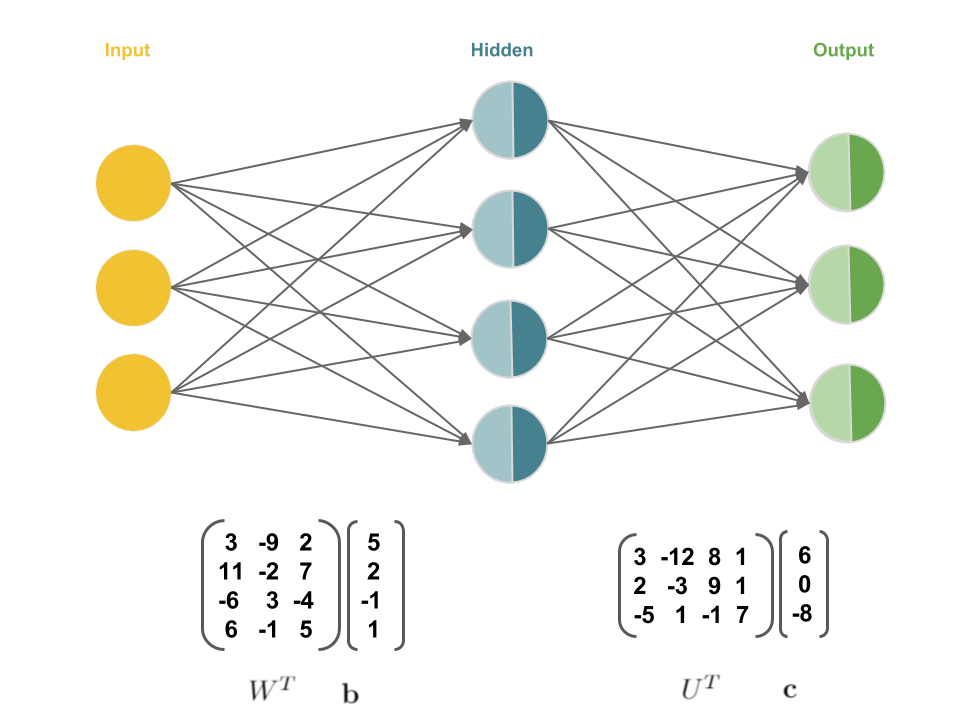
\includegraphics{figure/softie_one.png}}}
      \only<2>{\scalebox{0.95}{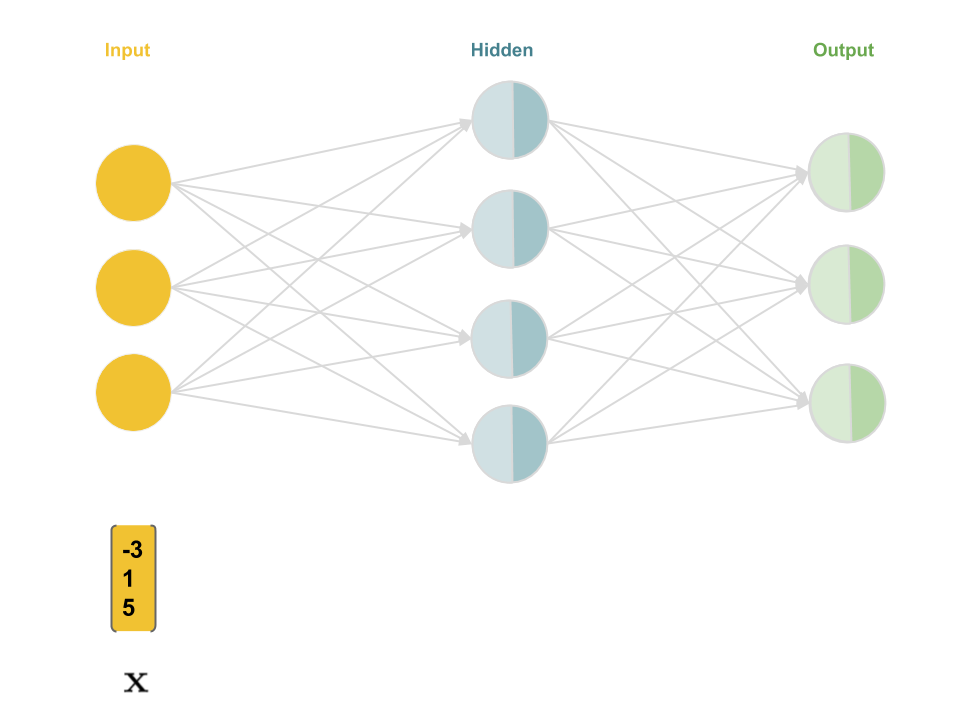
\includegraphics{figure/softie_two.png}}}
      \only<3>{\scalebox{0.95}{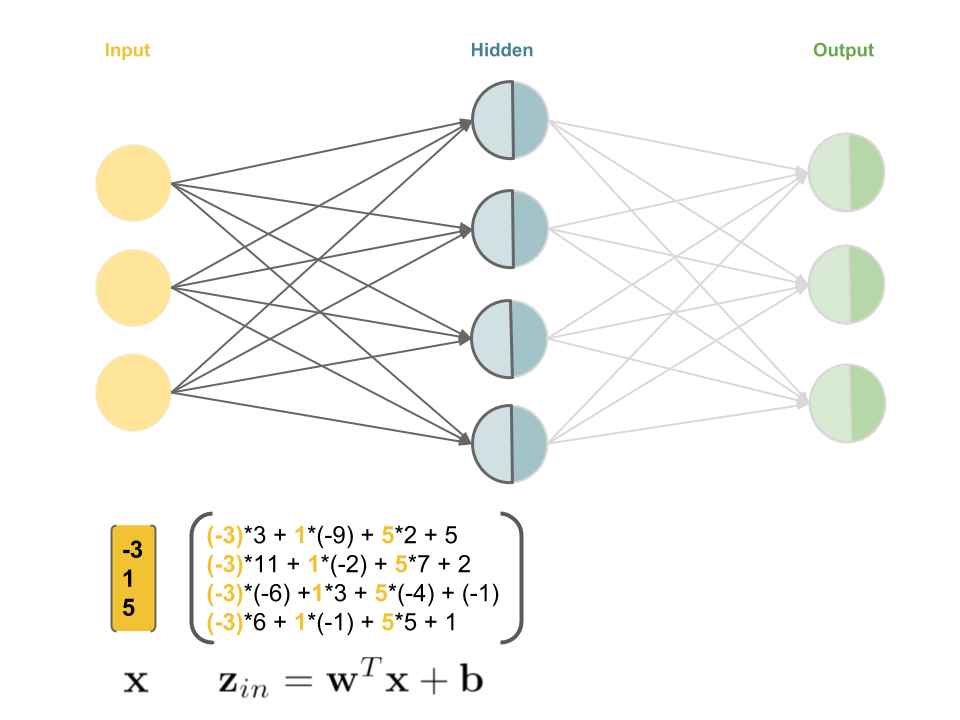
\includegraphics{figure/softie_three.png}}}
      \only<4>{\scalebox{0.95}{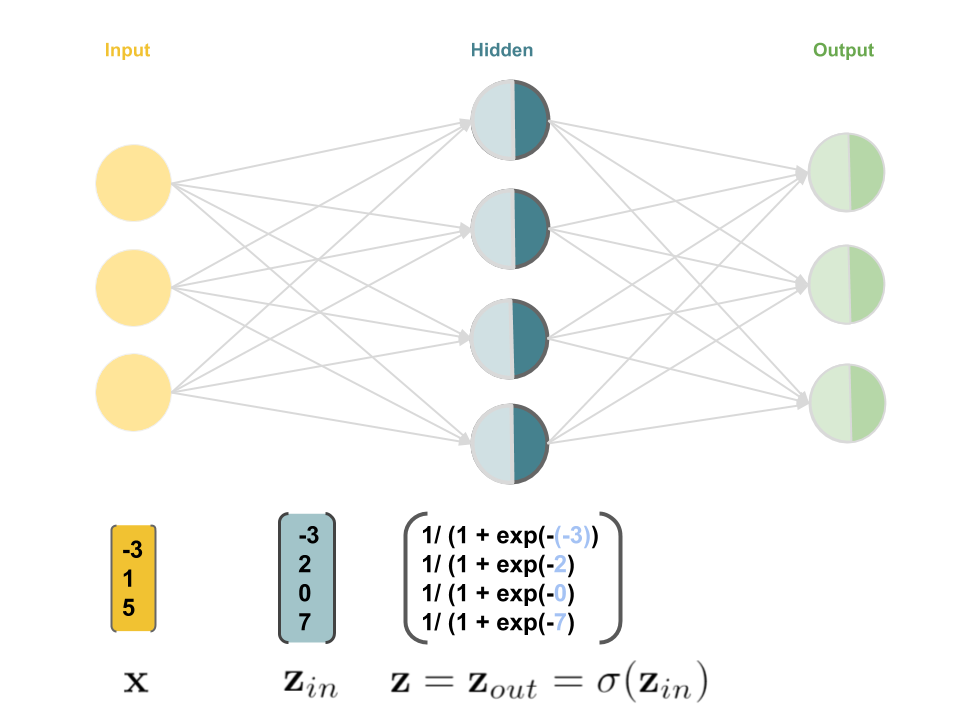
\includegraphics{figure/softie_four.png}}}
      \only<5>{\scalebox{0.95}{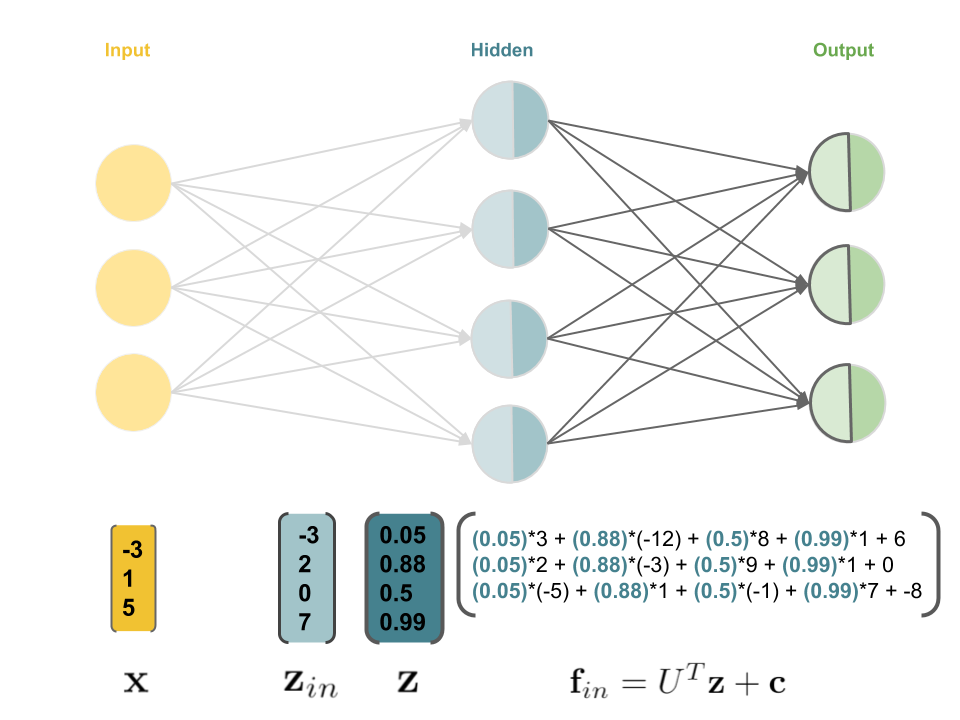
\includegraphics{figure/softie_five_a.png}}}
      \only<6>{\scalebox{0.95}{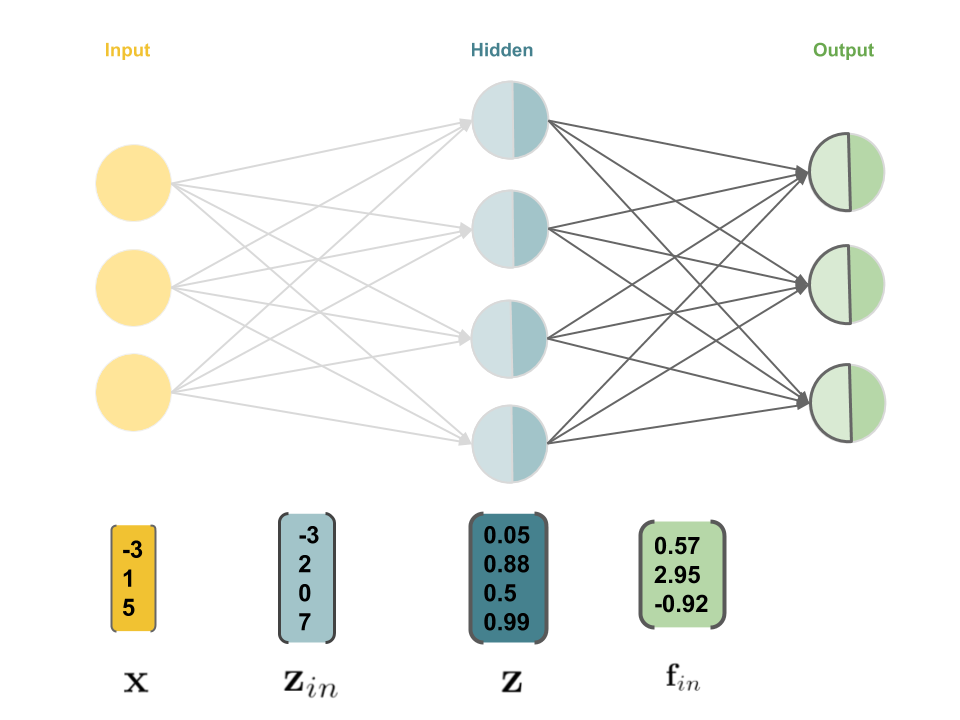
\includegraphics{figure/softie_five_b.png}}}
      \only<7>{\scalebox{0.95}{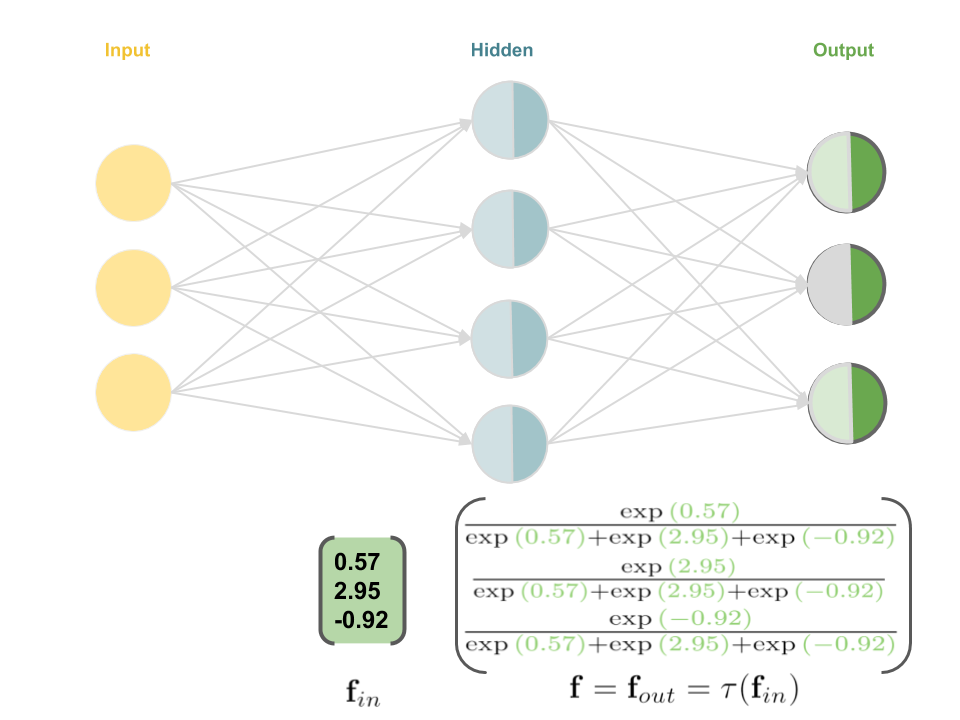
\includegraphics{figure/softie_six.png}}}
      \only<8>{\scalebox{0.95}{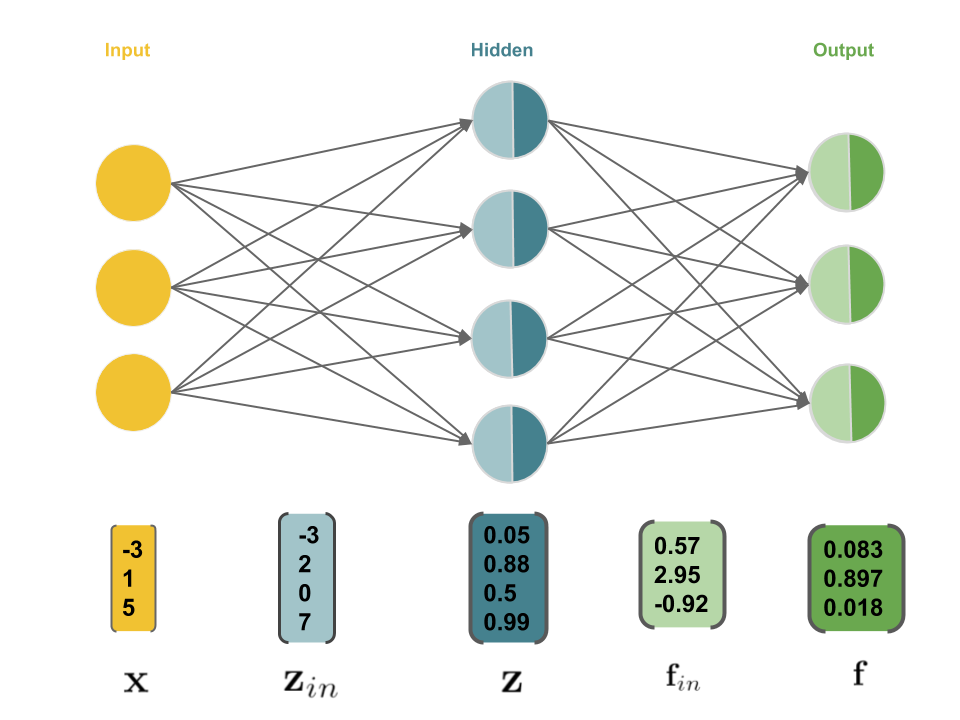
\includegraphics{figure/softie_seven.png}}}
\end{figure}
\end{frame}
%%%%%%%%%%%%%%%%%%%%%%%%%%%%%%%%%%%%%%%%%%%%%%%%%%%%%%%%%%%%%%%%%%

\begin{frame} {Softmax Loss}
  \begin{itemize}
\vspace{5mm}
\item The loss function for a softmax classifier is
$$L(y, \fx) = - \sum_{k = 1}^g [y = k] \log \left( \frac{\exp(f_{in,k})}{\sum_{k'=1}^g\exp(f_{in,k'})}\right)$$
where $[y = k] = \begin{cases} 1 & \text{ if } y = k \\
0 & \text{ otherwise }
\end{cases}$. 
\vspace{5mm}
\item This is equivalent to the cross-entropy loss when the label vector $\bm{y}$ is one-hot coded (e.g. $\mathbf{y} = (0,0,1,0)^\top$). 
\item Optimization:  Again, there is no analytic solution.
\end{itemize}
\end{frame}
%%%%%%%%%%%%%%%%%%%%%%%%%%%%%%%%%%%%%%%%%%%%%%%%%%%%%%%%%%%%%%%%%%

%%%%%%%%%%%%%%%%%%%%%%%%%%%%%%%%%%%%%%%%%%%%%%%%%%%%%%%%%%%%%%%%%%

\section{Multi-Layer Feedforward Neural Networks}
%%%%%%%%%%%%%%%%%%%%%%%%%%%%%%%%%%%%%%%%%%%%%%%%%%%%%%%%%%%%%%%%%%

\begin{vbframe}{Feedforward neural networks}
\begin{itemize}
\vspace{15mm}
\item We will now extend the model class once again, such that we allow an arbitrary amount of $l$ (hidden) layers.
\vspace{5mm}
\item The general term for this model class is (multi-layer) \textbf{feedforward networks} (inputs are passed through the network from left to right, no feedback-loops are allowed)
\end{itemize}
\framebreak
%%%%%%%%%%%%%%%%%%%%%%%%%%%%%%%%%%%%%%%%%%%%%%%%%%%%%%%%%%%%%%%%%%

\begin{itemize}
\item We can characterize those models by the following chain structure: $$f(\xv) = \tau \circ \phi \circ \sigma^{(l)} \circ \phi^{(l)} \circ \sigma^{(l-1)} \circ \phi^{(l-1)} \circ \ldots \circ \sigma^{(1)} \circ \phi^{(1)}$$ where $\sigma^{(i)}$ and $\phi^{(i)}$ are the activation function and the weighted sum of hidden layer $i$, respectively. $\tau$ and $\phi$ are the corresponding components of the output layer.
\vspace{5mm}
\item Each hidden layer has: 
\begin{itemize}
\vspace{2mm}
\item an associated weight matrix $\Wmat^{(i)}$, bias $\biasb^{(i)}$ and activations $\hidz^{(i)}$ for $i \in \{ 1 \ldots l\}$
\vspace{2mm}
\item $\hidz^{(i)} = \sigma^{(i)}(\phi^{(i)}) = \sigma^{(i)}(\Wmat^{(i)T}\hidz^{(i - 1)} + \biasb^{(i)})$ , where $\hidz^{(0)} = \xv$.
\end{itemize}
\vspace{5mm}
\item Again, without non-linear activations in the hidden layers, the network can only learn linear decision boundaries.
  \end{itemize}
\framebreak
%%%%%%%%%%%%%%%%%%%%%%%%%%%%%%%%%%%%%%%%%%%%%%%%%%%%%%%%%%%%%%%%%%

\lz
\begin{figure}
\centering
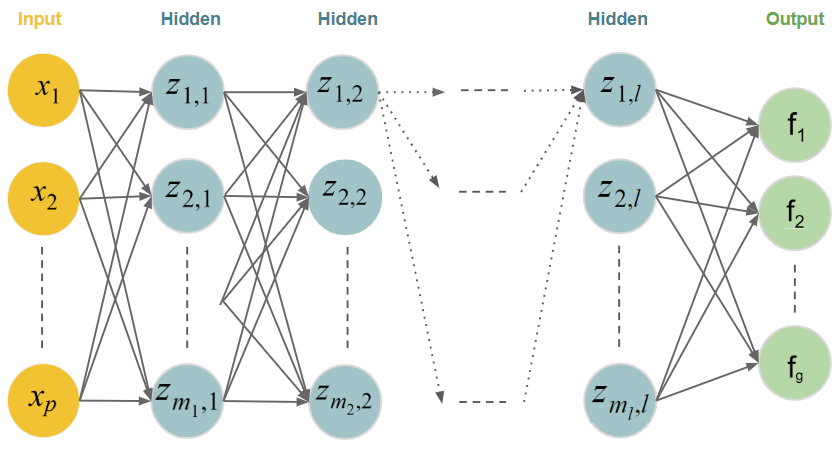
\includegraphics[width=10.5cm]{figure/deepneuralnet_new.png}
\caption{Structure of a deep neural network with $l$ hidden layers (bias terms omitted).}
  \end{figure}
\end{vbframe}  
%%%%%%%%%%%%%%%%%%%%%%%%%%%%%%%%%%%%%%%%%%%%%%%%%%%%%%%%%%%%%%%%%%

\begin{frame} {Feedforward neural networks: Example}
\begin{figure}
\centering
\only<1>{\scalebox{0.95}{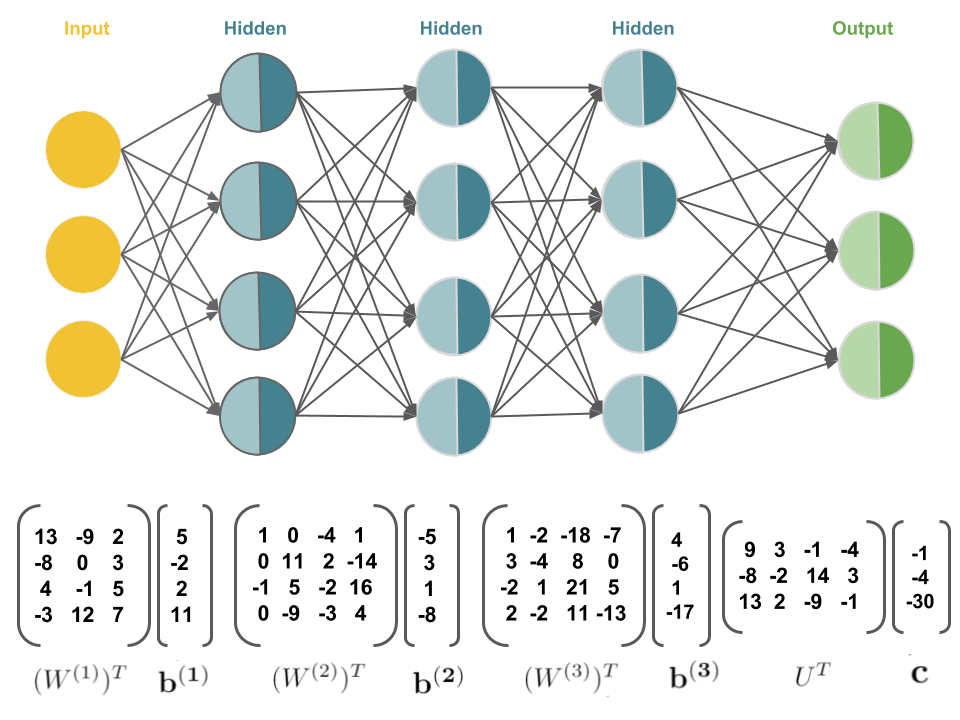
\includegraphics{figure/deepnet_one.png}}}
\only<2>{\scalebox{0.95}{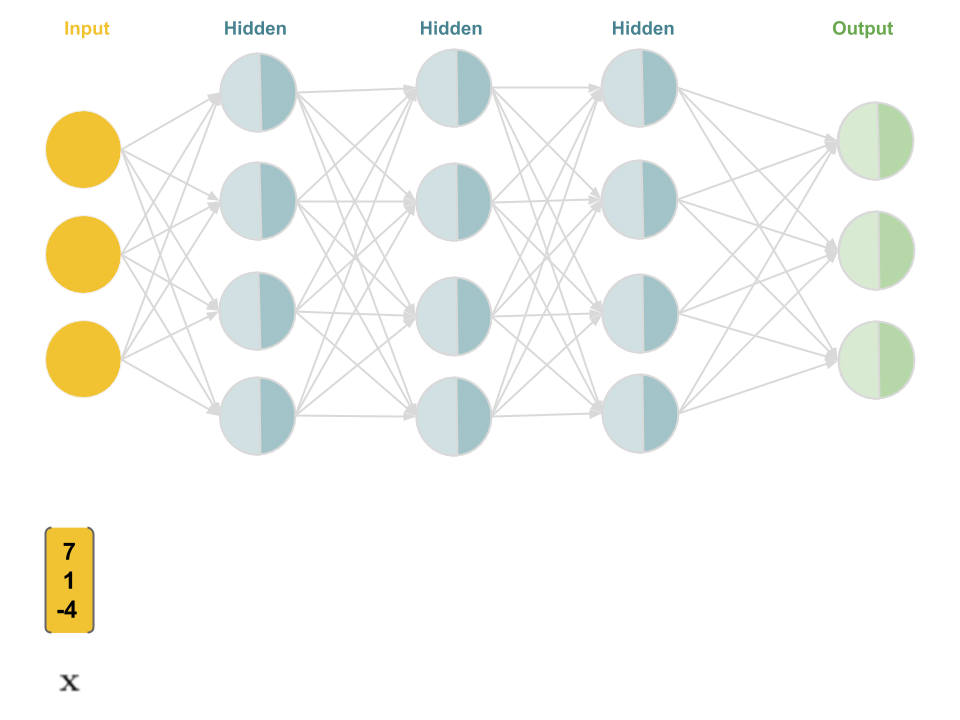
\includegraphics{figure/deepnet_two.png}}}
\only<3>{\scalebox{0.95}{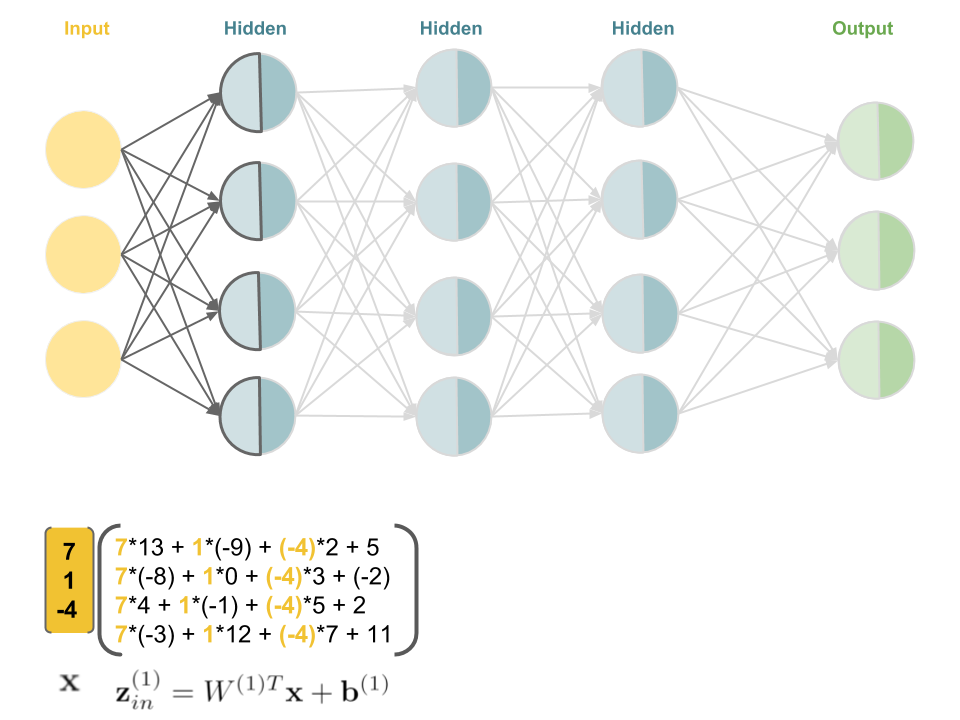
\includegraphics{figure/deepnet_three.png}}}
\only<4>{\scalebox{0.95}{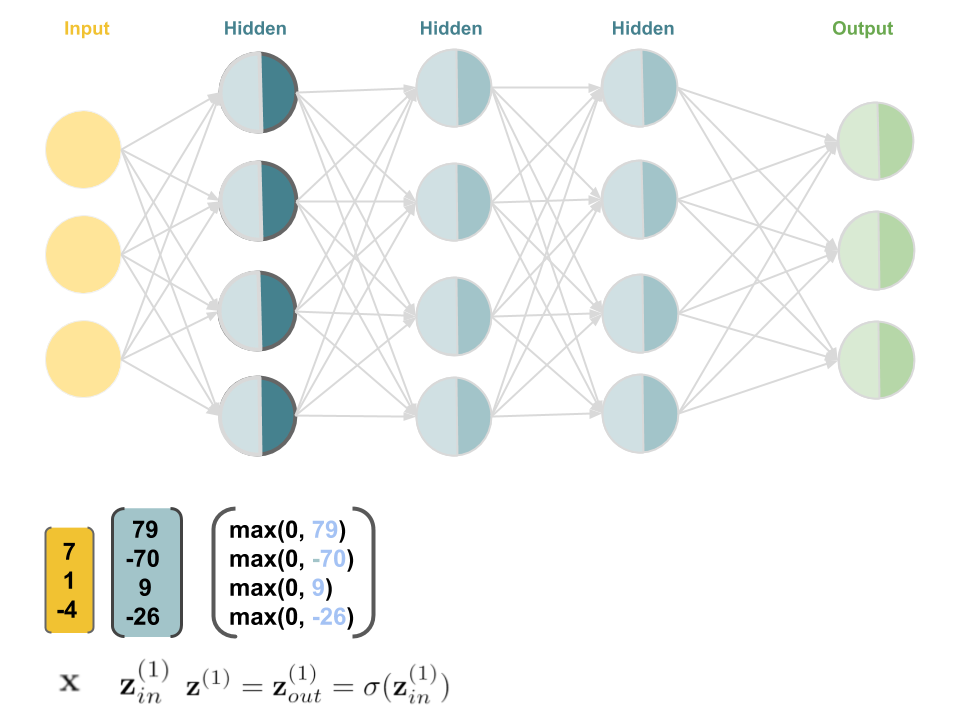
\includegraphics{figure/deepnet_four.png}}}
\only<5>{\scalebox{0.95}{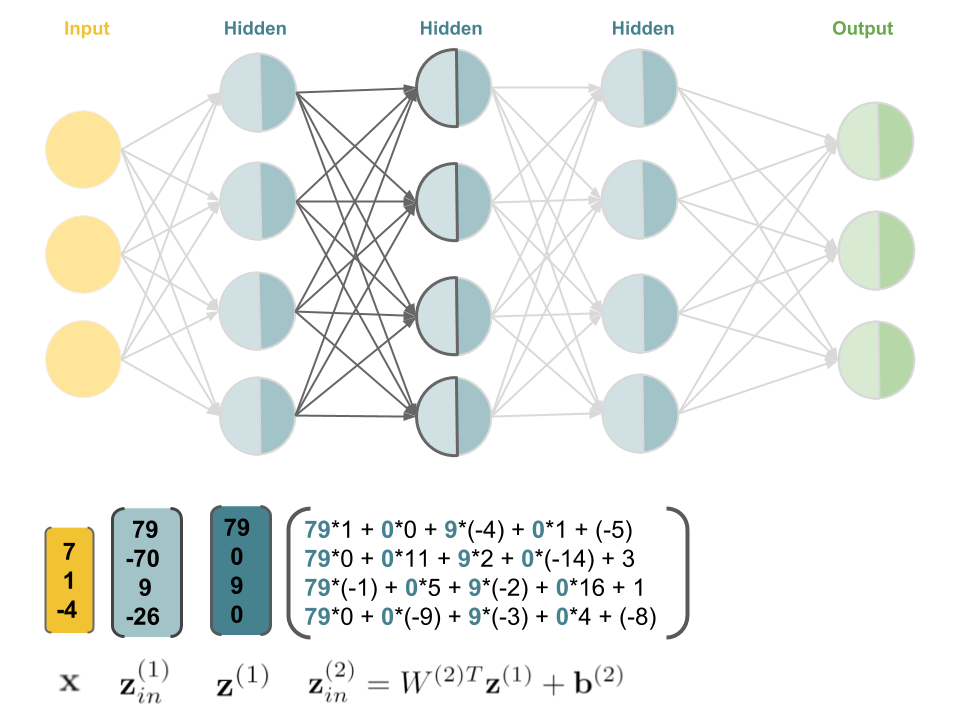
\includegraphics{figure/deepnet_five.png}}}
\only<6>{\scalebox{0.95}{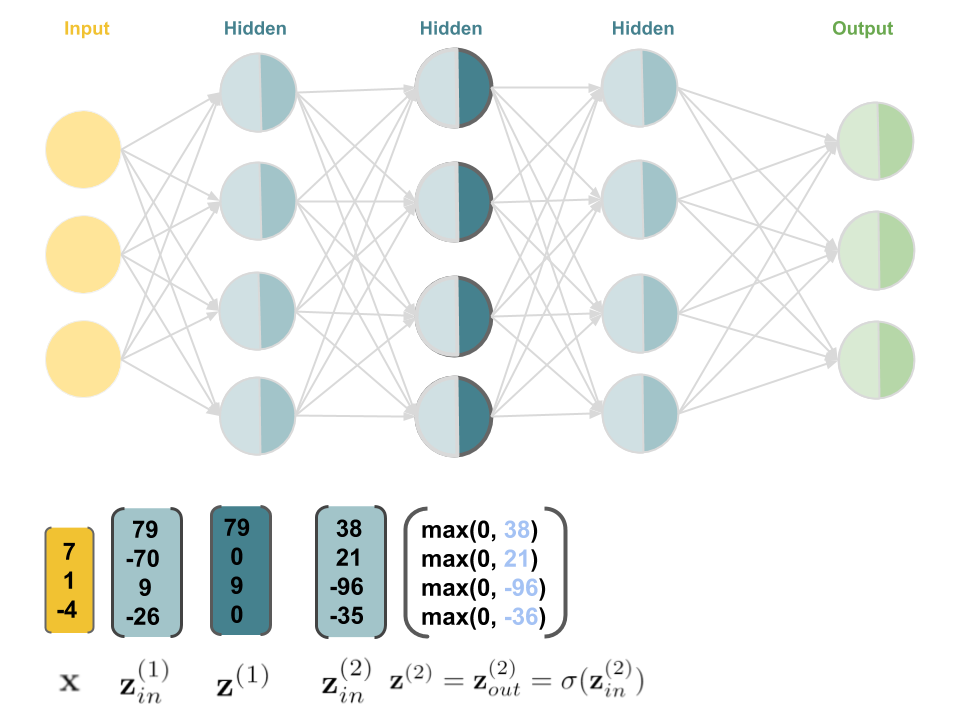
\includegraphics{figure/deepnet_six.png}}}
\only<7>{\scalebox{0.95}{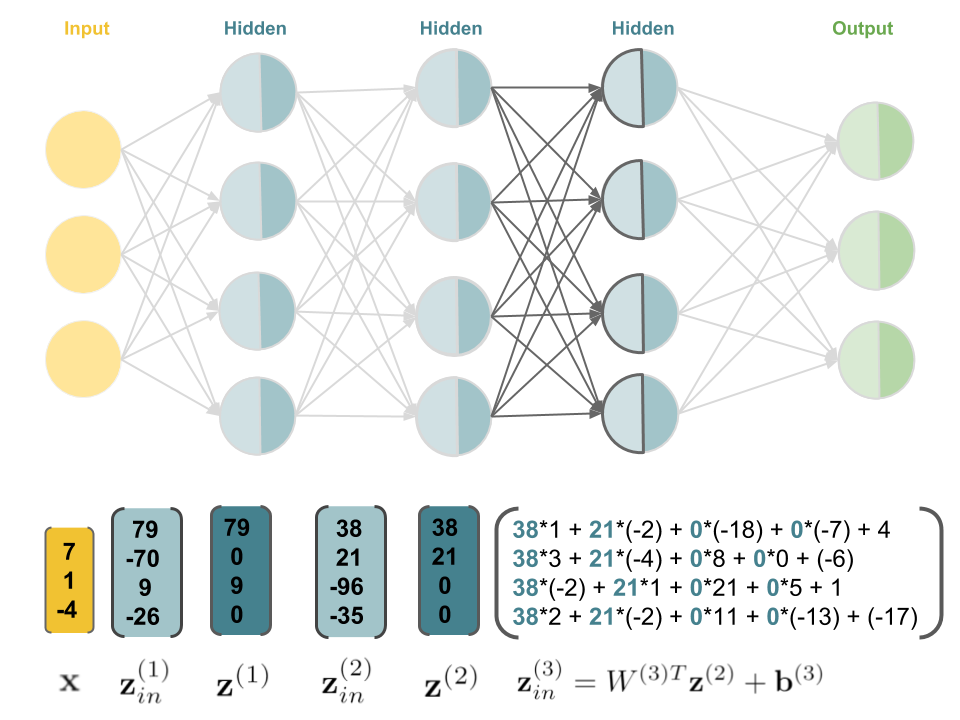
\includegraphics{figure/deepnet_seven.png}}}
\only<8>{\scalebox{0.95}{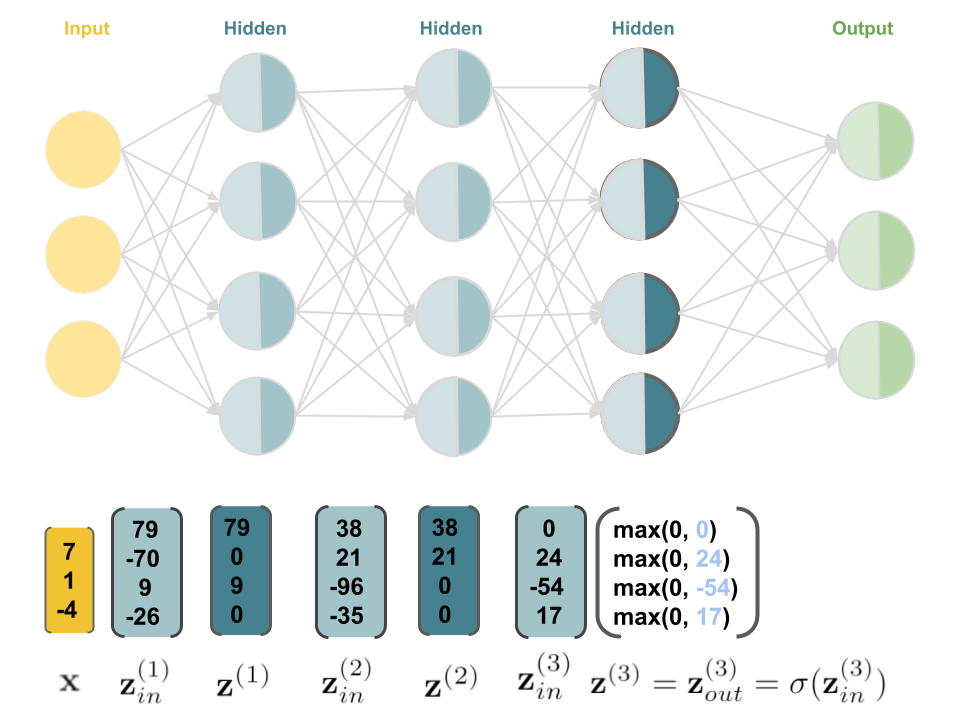
\includegraphics{figure/deepnet_eight.png}}}
\only<9>{\scalebox{0.95}{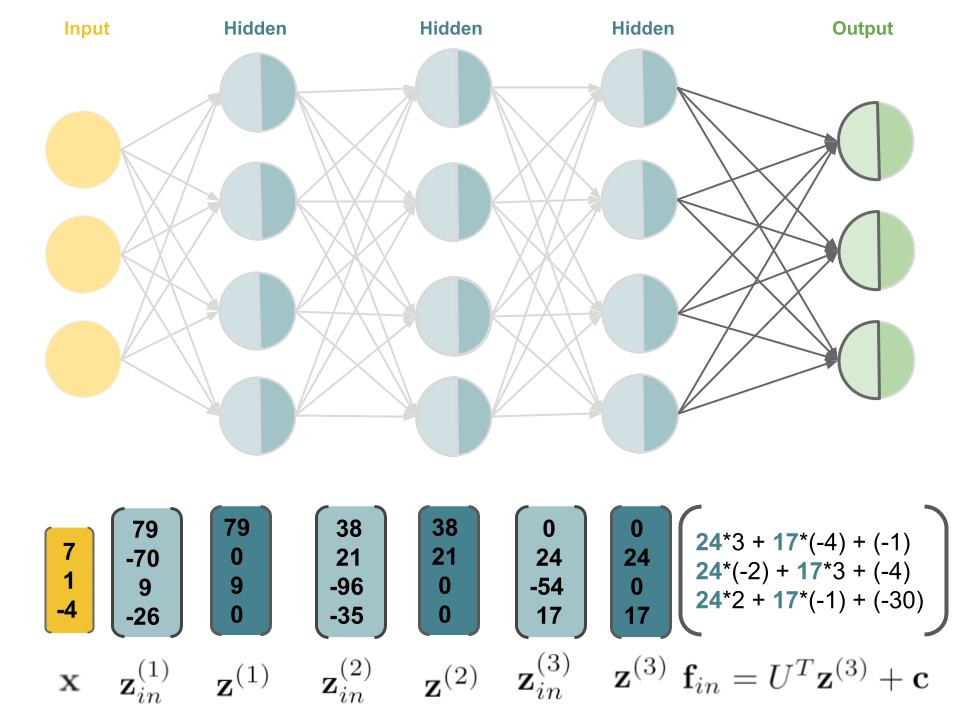
\includegraphics{figure/deepnet_nine.png}}}
\only<10>{\scalebox{0.95}{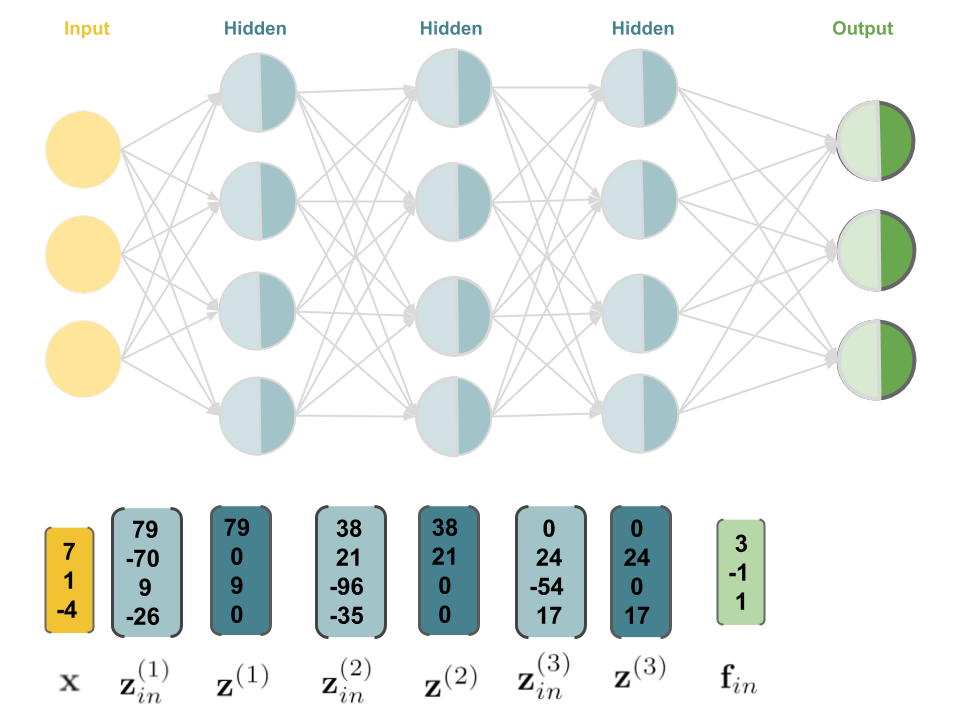
\includegraphics{figure/deepnet_ten.png}}}
\only<11>{\scalebox{0.95}{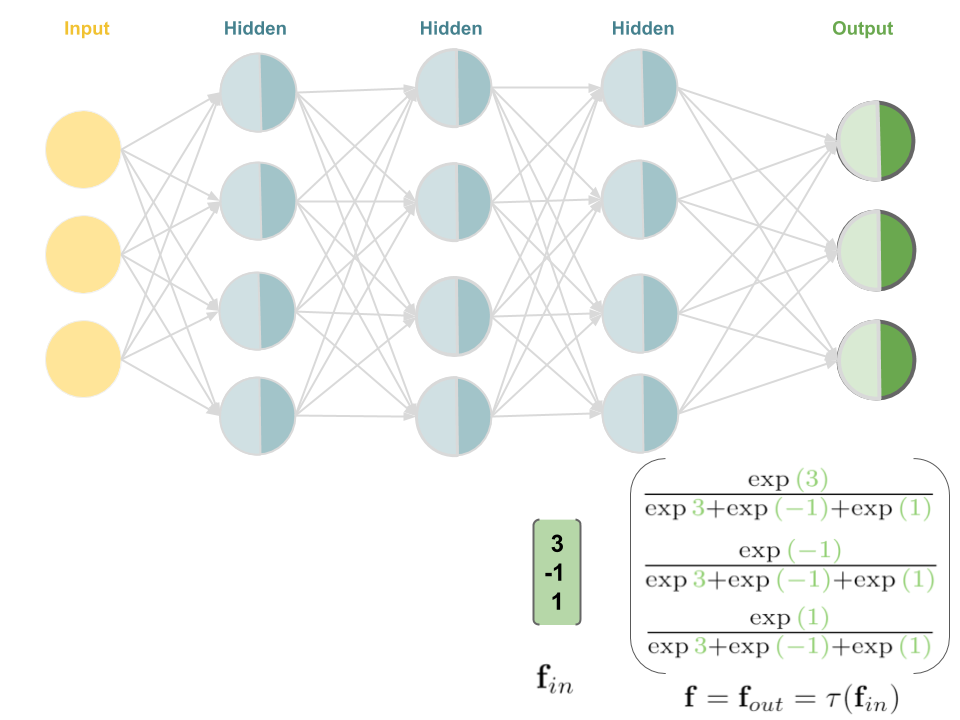
\includegraphics{figure/deepnet_eleven.png}}}
\only<12>{\scalebox{0.95}{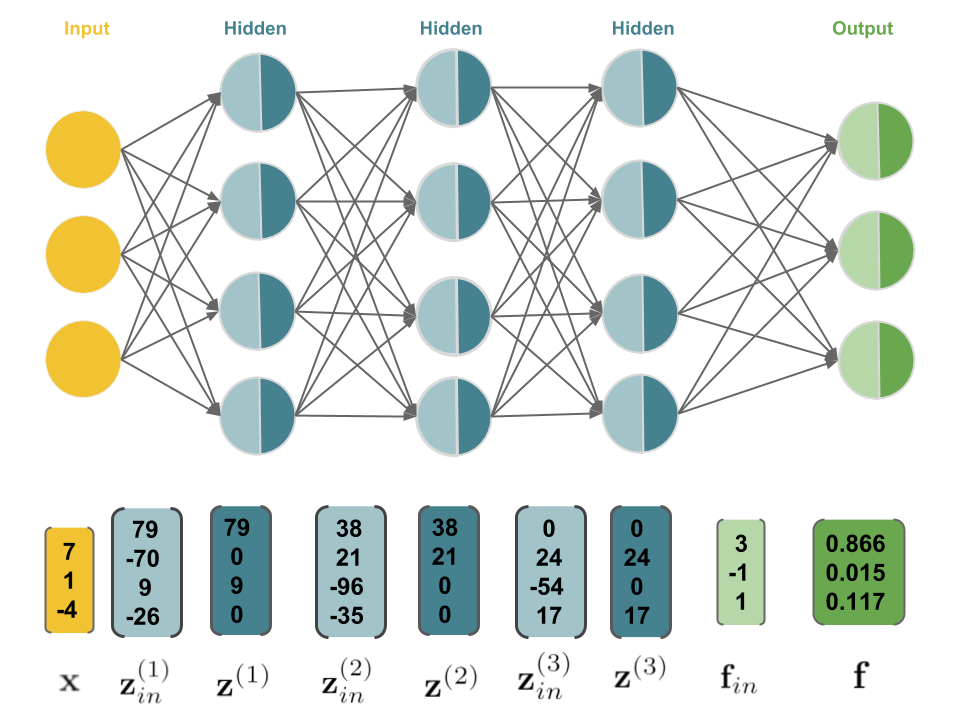
\includegraphics{figure/deepnet_twelve.png}}}
\end{figure}
\end{frame}
%%%%%%%%%%%%%%%%%%%%%%%%%%%%%%%%%%%%%%%%%%%%%%%%%%%%%%%%%%%%%%%%%%

\endlecture
\end{document}